\documentclass[10pt]{article}

% Pacotes extras necessários
\usepackage{amsmath}
\usepackage[lmargin=0.5in, rmargin=0.5in, tmargin=0.5in, bmargin=0.5in, includehead, includefoot]{geometry}
\usepackage{amsfonts}
\usepackage[utf8]{inputenc}
\usepackage[portuguese]{babel}
\usepackage{graphicx}
\usepackage{fancyhdr}
\usepackage{setspace}
\usepackage{listings}
\usepackage{url}
\usepackage{enumitem}

% More defined colors
\usepackage[dvipsnames]{xcolor}
 
% Required package
\usepackage{tikz}
\usetikzlibrary{positioning}

\graphicspath{ {./images/} }

% Sets para outras partes
\setlength{\parindent}{0pt}
\setstretch{1.5}
\DeclareMathOperator{\sen}{sen}
\DeclareMathOperator{\sinc}{sinc}

%% Facilidades
%% -- Laplace
\newcommand{\Lap}[1]{\mathcal{L}\left\{#1\right\}}

%% -- Negrito em matemáticas
\newcommand{\bm}[1]{\boldsymbol{#1}}


% ------- Estilo do trabalho -------- %
\fancypagestyle{capa}{
    \fancyhf{}
    \renewcommand\headrulewidth{0pt}
}

\pagestyle{fancy}
\fancyhead{}
\fancyhead[L]{\thepage}
\fancyfoot{}
% ----------------------------------- %

% Dados do Grupo
\title{Modelagem de Sistemas Dinâmicos - Trabalho Nº2}
\author{
    Leonardo Soares da Costa Tanaka - DRE: 121067652 \\
    Engenharia de Controle e Automação/UFRJ \\
    Rio de Janeiro, Brasil \\
    Junho de 2023
}
\date{}

\begin{document}
\maketitle
\thispagestyle{capa}

\quad Considerando um motor de corrente contínua (DC) controlado por corrente de armadura
com entrada de tensão $V_a(t)$ (V), saída de velocidade angular $\omega_m(t)$ (rad/s),
representado pelo circuito abaixo:

\begin{figure}[h]
    \centering
    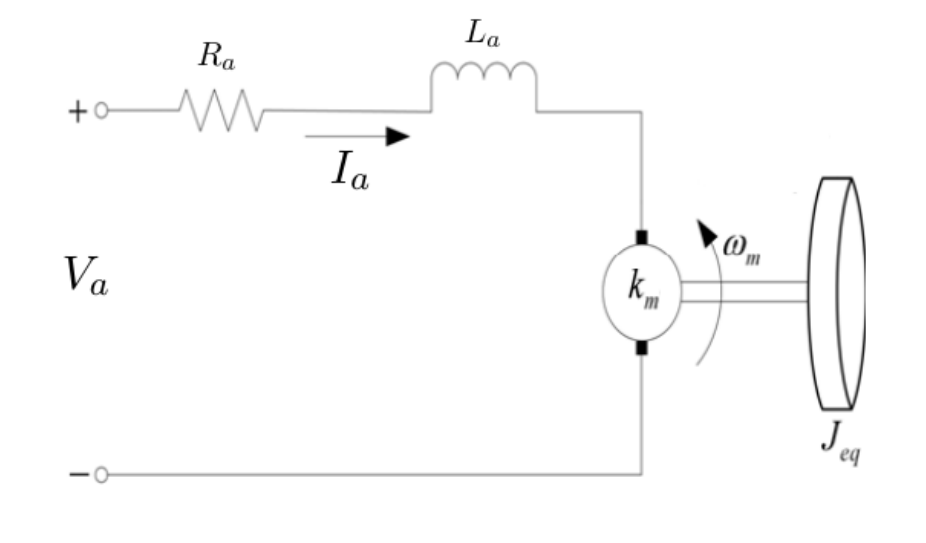
\includegraphics[scale=0.3]{circuito.png}
    \caption{Circuito}
\end{figure}

\quad O motor considerado tem as seguintes características dadas pelo fabricante:

\begin{itemize}[label={\textbullet}]
    \item Resistência de armadura: $R_a = 10.6 \Omega$
    \item Indutância de armadura: $L_a = 0.82 mH$
    \item Momento de Inércia do Rotor do Motor: $J_m = 1.16 \cdot  10^{-6} kgm^2$
    \item Constantes do Motor: $K_m = 0.0502 Nm/A$, $K_e = 0.0502 V s$
    \item Tensão máxima: 15 volts
    \item Massa do disco de inércia: $0.068 kg$
    \item Raio do disco de inércia: $0.0248 m$
\end{itemize}

\section{Modelagem teórica}

\quad Organizando as equações do sistema para obter o diagrama de blocos e a função de transferência.
Utilizando a Lei de Kirchhoff das Tensões, Equação do Torque, Lei do Motor e Lei do Gerador. Depois,
realizando a Transformada de Laplace das equações:

\begin{equation}
\begin{aligned}
    R_a \cdot i_a + L_a \frac{di_a}{dt} = V_a - e_c, \quad J_{eq} \frac{d\omega_m}{dt} = T_m, \quad T_m = K_m \cdot i_a, \quad e_c = K_e \cdot \omega_m \\
    I_a(s) = \frac{1/R_a}{\frac{L_a}{R_a}s + 1}(V_a(s) - e_c(s)), \quad \Omega(s) = \frac{1}{J_{eq} s }T_m(s), \quad T_m(s) = K_m \cdot I_a(s), \quad E_c(s) = K_e\Omega_m(s)
\end{aligned}
\end{equation}

\quad 1.1. Montando um diagrama de blocos do sistema (Desconsiderando o atrito do sistema).
O bloco azul é o subsistema elétrico, o bloco laranja é o subsistema mecânico e os blocos verdes são interligações entre o sistema elétrico e mecânico:

\begin{center}
\begin{tikzpicture}
 
    % Sum shape
    \node[draw,
        circle,
        minimum size=0.6cm,
        fill=white
    ] (sum) at (0,0){};
     
    \draw (sum.north east) -- (sum.south west)
        (sum.north west) -- (sum.south east);
     
    \draw (sum.north east) -- (sum.south west)
    (sum.north west) -- (sum.south east);
     
    \node[left=-1pt] at (sum.center){\tiny $+$};
    \node[below] at (sum.center){\tiny $-$};
     
    % corrente
    \node [draw,
        fill=cyan,
        minimum width=2cm,
        minimum height=1.2cm,
        right=1cm of sum
    ]  (corrente) {$\frac{1/R_a}{\frac{L_a}{R_a}s + 1}$};

    % torque
    \node [draw,
        fill=lime,
        minimum width=2cm,
        minimum height=1.2cm,
        right=1cm of corrente
    ]  (torque) {$K_m$};
     
    % velocidade
    \node [draw,
        fill=orange, 
        minimum width=2cm, 
        minimum height=1.2cm,
        right=1cm of torque
    ] (velocidade) {$\frac{1}{J_{eq} s}$};
     
    % eletromotriz
    \node [draw,
        fill=lime, 
        minimum width=2cm, 
        minimum height=1.2cm, 
        below right= 1cm and -2cm of torque
    ]  (eletromotriz) {$K_e$};
     
    % Arrows with text label
    \draw[-stealth] (sum.east) -- (corrente.west);

    \draw[-stealth] (corrente.east) -- (torque.west) 
        node[midway,above]{$I_a$};
     
    \draw[-stealth] (torque.east) -- (velocidade.west) 
        node[midway,above]{$T_m$};
     
    \draw[-stealth] (velocidade.east) -- ++ (1.25,0) 
        node[midway](output){}node[midway,above]{$\Omega_m$};
     
    \draw[-stealth] (output.center) |- (eletromotriz.east);
     
    \draw[-stealth] (eletromotriz.west) -| (sum.south) 
        node[near end,left]{$E_c$};
     
    \draw (sum.west) -- ++(-1,0) 
        node[midway,above]{$V_a$};
     
\end{tikzpicture}
\end{center}

\quad 1.2. Calculando a função de transferência do motor $G(s)$ de $V_a(s)$ para $\Omega_m(s)$
(Levando em consideração que é um sistema realimentado):

\begin{equation}
    G(s) = \frac{\Omega_m(s)}{V_a(s)}
    = \frac{\frac{K_m}{R_a \cdot J_{eq}}\frac{1}{s (\frac{L_a}{R_a}s + 1)}}{1 + \frac{K_e \cdot K_m}{R_a \cdot J_{eq}}\frac{1}{s (\frac{L_a}{R_a}s + 1)}}
    = \frac{k_m}{R_a \cdot J_{eq} \cdot s \cdot (\frac{L_a}{R_a}s + 1) + K_e \cdot K_m}
    = \frac{\frac{k_m}{J_{eq} \cdot L_a}}{s^2 + \frac{R_a}{L_a}s + \frac{K_e \cdot K_m}{J_{eq} \cdot L_a}}
    = \frac{\frac{1}{K_e}}{}
\end{equation}

\quad 1.3. Representando o sistema no espaço de estados com a realização canónica controlável:

\begin{equation}
\begin{aligned}
    \dot{x} =
    \begin{bmatrix}
        0 && 1 \\
        -\frac{K_e \cdot K_m}{J_{eq} \cdot L_a} && -\frac{R_a}{L_a}
    \end{bmatrix} x
    +
    \begin{bmatrix}
        0 \\
        1
    \end{bmatrix}
    u \\
    y =
    \begin{bmatrix}
        \frac{k_m}{J_{eq} \cdot L_a} && 0
    \end{bmatrix} x
\end{aligned}
\end{equation}

\quad 1.4. Calculando a inércia do disco (feito de alumínio):

\begin{equation}
\begin{aligned}
    J = \int r^2 dm
    ,\quad \frac{dm}{M} = \frac{dA}{A} = \frac{2 \pi r dr}{\pi R^2}
    ,\quad J_d = \int_{0}^{R} \frac{r^2 M 2 \pi r}{\pi R^2} dr
    = \frac{2M}{R^2} \int_{0}^{R} r^3 dr
    = \frac{2Mr^4}{4R^2} \Bigg|_{0}^{R}
    = \frac{MR^2}{2} \\
    J_d = \frac{0.068 \cdot 0.0248^2}{2} = 20.91136 \ 10^{-6} \ kgm^2
\end{aligned}
\end{equation}

\quad Determinando momento de inércia total (rotor e disco),
levando em consideração que estão conectadas no mesmo eixo de rotação e
estão perfeitamente fixadas juntas. Podemos usar a seguinte fórmula e valores:

\begin{equation}
    J_{eq} = J_m + J_d = (1.16 \ 10^{-6} + 20.91136 \ 10^{-6}) \ kgm^2
    = 22.07136 \ 10^{-6} \ kgm^2
\end{equation}

\quad 1.5. Considerando que a função de transferência G(s) tenha a seguinte estrutura:

\begin{equation}
    G(s) = \frac{K}{(\tau_e s + 1)(\tau_m s + 1)}
\end{equation}

\quad Utilizando a equação (2) e as características dadas pelo fabricante para calcular
os pólos da função de transferência:

\begin{equation}
\begin{aligned}
    p_{1,2} = \frac{-\frac{R_a}{L_a} \pm \sqrt{\frac{R_a^2}{L_a^2} - 4\frac{K_e \cdot K_m}{J_{eq} \cdot L_a}}}{2}
    = \frac{-\frac{10.6}{0.82 \cdot 10^{-3}} \pm \sqrt{\frac{10.6^2}{(0.82 \cdot 10^{-3})^2} - 4\frac{0.0502 \cdot 0.0502}{22.07136 \ 10^{-6} \cdot 0.82 \cdot 10^{-3}}}}{2}
    = \frac{-12926.82927 \pm 12905.26847}{2} \\
    p_1 = -12916.04887, \quad p_2 = -10.7804 \\
    K = \frac{k_m}{J_{eq} \cdot L_a \cdot p_1 \cdot p_2} = 19.92031563, \quad \tau_e = -\frac{1}{p_1} = 7.742305794 \ 10^{-5}, \quad \tau_m = -\frac{1}{p_2} = 0.09276093651
\end{aligned}
\end{equation}

\quad A constante de tempo elétrica $\tau_e$ pode ser considerada despressível
comparada com a constante de tempo mecânica $\tau_m$,
porque a constante de tempo elétrica é pequena em relação aos tempos de interesse,
isso significa que o sistema tem uma dinâmica inicial rápida devido ao polo rápido,
mas em seguida, a resposta se estabiliza gradualmente devido ao polo lento.
O efeito do polo lento será mais predominante à medida que o tempo avança.

\quad 1.6. Considerando que não existe perturbação nem atrito,
é possível determinar a velocidade máxima do motor $\omega_{max}$:

\begin{equation}
    e_{max} = K_e \cdot \omega_{max},
    \quad \omega_{max} = \frac{e_{max}}{K_e} = \frac{15}{0.0502} = 298.8047809 \ rad/s
\end{equation}

\quad 1.7. Determinando a corrente máxima $I_{max}$ utilizando Lei de Ohm e máximo de torque gerado $T_{max}$ utilizando Lei do Gerador:

\begin{equation}
    I_{max} = \frac{e_{max}}{R_a} = \frac{15}{10.6} = 1.4150943396 \ A, \quad T_{max} = K_m I_{max} = 0.0502 \cdot 1.4150943396 = 0.0710377358 \ Nm
\end{equation}

\section{Identificação Experimental}

\quad 2.1. Determinando experimentalmente no kit QET da Quanser, de forma estatística,
as constantes utilizadas como parâmetros na modelagem teórica:

\quad (a) Aplicando voltagem constante $V_a$ e medindo a corrente $I_a$,
levando em consideração que é mantido o eixo do motor parado
e que o indutor de armadura se torna um curto-cicuito no momento da medição.
Foi utilizado os dados obtidos experimentalmente para realizar uma Regressão Linear em Python com Scikit-Learn
para obter o valor estimado da Resistência de armadura $R_a$:

\begin{verbatim}
    import numpy as np
    from sklearn.linear_model import LinearRegression
    # Dados de voltagem Va(V) em Volts e corrente Ia(A) que foram enviados em forma de tabela
    voltagem = np.array([1.0, 2.0, 3.0, 4.0, 4.9, 5.9, 6.9, 7.9, 8.9, 9.9])
    corrente = np.array([0.076, 0.150, 0.225, 0.305, 0.425, 0.474, 0.550, 0.620, 0.720, 0.800])
    # Ajuste da regressão linear
    x = corrente.reshape(-1, 1)  # Converte corrente para formato adequado
    y = voltagem
    regressor = LinearRegression()
    regressor.fit(x, y)
    # Estimativa da resistência média (coeficiente angular da regressão linear)
    resistencia_media = regressor.coef_[0]
    # Exibindo os resultados
    print("Resistência média:", resistencia_media, "ohms")
\end{verbatim}

Valor estimado da Resistência de armadura $R_a$: 12.222223261373172 $\Omega$

\quad (b) Aplicando voltagem constante $V_a$ e medindo corrente e velocidade.
Considerando que a resistência de armadura é conhecida. Foi utilizado os dados obtidos
experimentalmente para realizar uma Regressão Linear em Python com Scikit-Learn
para obter o valor estimado da Constante de torque do motor $K_m$:

\begin{verbatim}
    import numpy as np
    from sklearn.linear_model import LinearRegression
    # Ra resistência de armadura
    Ra = 10.6
    Jeq = Jeq = 22.07136 * 10**(-6)
    # Dados de voltagem Va(V) em Volts, velocidade angular wm(rad/s) e corrente Ia(mA)
    Va = np.array([1.0, 2.0, 3.0, 4.0, 4.9, 5.9, 6.9, 7.9, 8.9, 9.9])
    wm = np.array([12, 29, 49, 70, 89, 105, 127, 148, 168, 185])
    Ia = np.array([1, 1, 1, 1, 1, 1, 2, 2, 2, 3])
    # Ajuste da regressão linear
    x = wm.reshape(-1, 1)  # Converte corrente para formato adequado
    y = Va - Ra * Ia * 10**(-3)
    regressor = LinearRegression()
    regressor.fit(x, y)
    # Estimativa da resistência média (coeficiente angular da regressão linear)
    constante_torque = regressor.coef_[0]
    # Exibindo os resultados
    print("Constante de torque do motor:", constante_torque, "Nm/A")
\end{verbatim}

\quad Valor estimado do Constante de Torque do motor $K_m$: 0.05048676538284488 Nm/A

\quad 2.2. Calculando a função de transferência do sistema G(s) com os parâmetros $\{ R_a, K_m \}$
estimados acima. Determinando os parâmetros $\{K,\tau_e, \tau_m\}$:

\begin{equation}
\begin{aligned}
    G(s) = \frac{\frac{k_m}{J_{eq} \cdot L_a}}{s^2 + \frac{R_a}{L_a}s + \frac{K_e \cdot K_m}{J_{eq} \cdot L_a}} = \frac{2789552.89}{s^2 + 14905.15032 \ s + 140835.5023} = \\
    K = 4.951792773, \quad \tau_e = 3.356674407 \ 10^{-5}, \quad \tau_m = 0.05288331173 
\end{aligned}
\end{equation}

\section{Validação dos modelos}

\quad Foram obtidas experimentalmente as respostas (rad/s) ao degrau (2, 4 e 10 volts) e
senoidal (5 volts).

\end{document}